
Fairness partial $\rho$ under MMLU versus Winogrande covariate:

\begin{table}[htbp]
\centering
\resizebox{\columnwidth}{!}{%
\begin{tabular}{llll}
\toprule
Covariate & Partial $\rho$ & N & p-value \\
\midrule
MMLU & 0.962 & 16 & < 0.0001 \\
Winogrande & 0.969 & 14 & < 0.0001 \\
\bottomrule
\end{tabular}
}
\end{table}

The fairness result is robust to covariate choice. Two models lack Winogrande scores (Koala-13B, OpenAssistant-12B), reducing N from 16 to 14 in the Winogrande analysis.

For $\Delta\rho$, Winogrande control yields $\Delta\rho$ = 0.073, substantially below MMLU $\Delta\rho$ = 0.192. The fairness-robustness differential is sensitive to covariate choice. Robustness $\rho$ values under Winogrande ($\rho_{AdvGLUE}$ = 0.886, $\rho_{ANLI}$ = 0.915) are higher than under MMLU (0.868, 0.684), suggesting that MMLU and Winogrande capture different components of general capability that interact differently with robustness-dimension variance. Richer capability covariates would clarify whether the MMLU $\Delta\rho$ finding is replicated under alternative controls.

\begin{figure}[htbp]
\centering
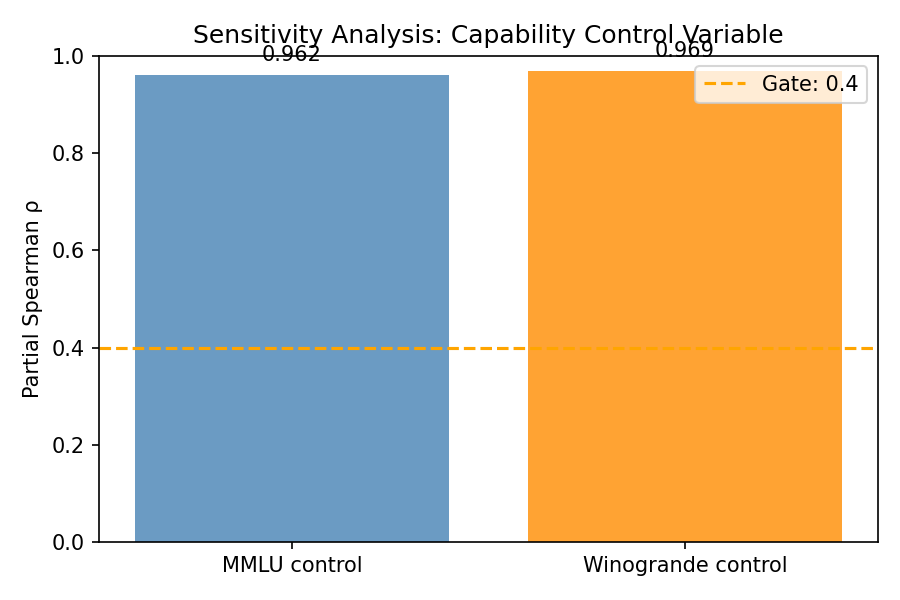
\includegraphics[width=\columnwidth]{figures/sensitivity_comparison.png}
\caption{Sensitivity comparison}
\label{fig:sensitivity_comparison}
\end{figure}

\textit{Figure 5. Fairness partial $\rho$ under MMLU (N = 16) versus Winogrande (N = 14) covariate. Results are near-identical for fairness; $\Delta\rho$ collapses substantially under Winogrande control.}

